\chapter{TINJAUAN PUSTAKA}
\label{chap:tinjauanpustaka}

\section{Penelitian Terdahulu}
\label{sec:penelitianterdahulu}

Finanta Okmuyura, Noverta Effendi, Witri Ramadhani, dan Adlian Jefiza melakukan penelitian ini dengan membuat analisis dan desain untuk dapat memonitor pembakaran kalori saat jogging. Pada penelitian ini, dalam memonitor pembakaran kalori menggunakan sensor akselerometer yang dapat menghitung berdasarkan dari tekanan dari beban yang diterima untuk menghasilkan nilai \emph{threshold} untuk dikalkukasikan nantinya. Perhitungan kalori yang terbakar pada penelitian ini dengan menggunakan nilai jumlah langkah kaki, waktu dan berat pengguna untuk memberikan informasi pembakaran kalori dalam jogging (Okmuyura et al., 2019).

Dina Budhi Utami dan Muhammad Ichwan melakukan penelitian mengenai sistem prediksi kalori yang terbakar pada pesepeda menggunakan \emph{Feedforward Neural Network}. Penelitian ini melakukan prediksi berdasarkan detak jantung dan kecepatan kayuh saat bersepeda. Model prediksi kalori yang digunakan adalah \emph{Feedforward Neural Network} dengan arsitektur jaringan saraf tiruan terdiri dari 3 lapis. Hasil keluaran dari jaringan saraf tiruan adalah nilai prediksi kalori menggunakan pengujian 10000 data latih dengan memiliki tingkat kesalahan adalah 7\% (Utami \& Ichwan, 2017).

Pada tahun 2019, Philip Saponaro bersama Haoran Wei, Gregory Dominick dan Chandra Kambhamettu melakukan penelitian ini. Penelitian yang dilakukan mengenai perkirakan intensitas aktivitas fisik dan pengeluaran energi dengan menggunakan sistem visi komputer. Nilai perkiraan aktivitas fisik dan pengeluaran energi menggunakan faktor usia, jenis kelamin, kecepatan dan isyarat aktivitas. Data nilai usia dan jenis kelamin didapatkan dengan jaringan \emph{Deep Expectation} dan nilai aktivitas diperoleh dari perkiraan sudut sendi dan kecepatan gerak. Hasil yang didapat dengan akurasi nilai perkiraan aktivitas fisik sebesar 89,5\% dan perbedaan rata-rata pengeluaran energi sebesar 1,96 kCal/min (Saponaro et al.,  2019).


\section{Kalori}
\label{sec:kalori}

Kalori adalah unit pengukuran yang mengukur kandungan energi makanan. Saat kita mengonsumsi makanan dan minuman, kita menyuplai tubuh dengan kalori atau energi. Kalori ini digunakan oleh tubuh untuk menggerakkan berbagai aktivitasnya. Semakin besar tingkat aktivitas fisik, semakin tinggi jumlah kalori atau energi yang dibutuhkan. Item makanan biasanya diberi label dengan informasi kalori yang dinyatakan dalam kilokalori (kkal). Kalori memainkan peran penting dalam menopang tubuh kita dan memfasilitasi berbagai aktivitas (Inmawati N. D., 2016).

Perhitungan kebutuhan kalori memperhitungkan berbagai faktor seperti jenis kelamin, usia, tinggi badan, berat badan, komposisi tubuh, tingkat aktivitas, dan kondisi fisik. Pria dan wanita memiliki kebutuhan kalori yang berbeda, bahkan dalam rentang usia yang sama. Jika seseorang melakukan aktivitas fisik yang sangat berat, asupan kalori hariannya perlu ditingkatkan. Memahami kebutuhan energi harian seseorang sangat penting untuk menjaga kesehatan secara keseluruhan karena mempengaruhi keseimbangan energi sepanjang hari. Pasar menyaksikan peningkatan ketersediaan pilihan makanan dengan kandungan kalori rendah, yang sering disebut sebagai "rendah lemak". Namun, banyak orang berjuang untuk mempertimbangkan pertimbangan kalori ini secara memadai dalam pilihan diet mereka.

Menghitung kalori secara akurat memang menantang karena beberapa faktor, antara lain berat badan, intensitas aktivitas, kondisi tubuh, dan metabolisme. Aktivitas fisik menyebabkan pengeluaran energi dalam tubuh. Jika asupan kalori melebihi energi yang dibakar melalui aktivitas fisik yang seimbang, maka dapat mengakibatkan kenaikan berat badan. Seiring bertambahnya usia, mereka cenderung menjadi kurang aktif secara fisik, mengalami penurunan massa otot, dan mengalami penurunan laju pembakaran kalori. Hal ini dapat mempersulit tubuh untuk membakar kalori yang dikonsumsi, yang menyebabkan akumulasi energi dan berpotensi menyebabkan obesitas. Seiring bertambahnya usia dan asupan kalori yang konsisten, kemampuan tubuh untuk membakar kalori yang masuk semakin berkurang, sehingga memengaruhi pengelolaan berat badan (Widiantini et al., 2013).

\section{\emph{Metabolic Equivalent of Task}}
\label{sec:met}

Catatan \emph{physical activity} memberikan perkiraan \emph{energy expenditure} (EE) berdasarkan laporan terperinci dari semua hasil harian terhadap \emph{physical activity} (PA) yang dilakukan. Namun, catatan-catatan ini sering dianggap sebagai metode pelengkap karena subjektivitasnya. Data PA dikategorikan dan dikodekan berdasarkan jenis dan intensitas aktivitas, memungkinkan deskripsi pola aktivitas fisik dalam suatu populasi dan eksplorasi faktor yang mempengaruhi pola tersebut. Selain itu, catatan ini memungkinkan penyelidikan hubungan antara aktivitas fisik, kesehatan, dan penyakit. Mereka juga dapat digunakan untuk menilai kontribusi berbagai jenis aktivitas fisik terhadap pengeluaran energi total (TEE), yang menawarkan wawasan tambahan tentang jenis aktivitas yang biasanya dilakukan. Salah satu sistem pengkodean yang tersedia adalah The Compendium of Physical Activity, yang diterbitkan pada tahun 1993 (Ainsworth et al., 1993). Kompendium ini menggunakan kode lima digit untuk mewakili aktivitas tertentu yang dilakukan dalam berbagai situasi. Setiap aktivitas dikaitkan dengan tingkat intensitas yang sesuai, yang dinyatakan dalam unit \emph{Metabolic Equivalent of Task} (MET)(Pinheiro et al., 2011).

\emph{Metabolic Equivalent of Task} (MET) adalah pengukuran yang menghitung jumlah oksigen yang dibutuhkan selama istirahat per kilogram berat badan dan waktu. Konsumsi oksigen pada \emph{Basal Metabolic Rate} (BMR) umumnya diperkirakan sekitar 3,5 mL O2/kg/menit, tetapi faktor seperti usia, jenis kelamin, dan penyakit dapat mempengaruhi nilai ini. Istilah "konsumsi oksigen relatif" (VO2 relatif) digunakan untuk menggambarkan nilai ini karena diberikan per kilogram massa tubuh. Mengalikannya dengan massa tubuh memberikan "konsumsi oksigen absolut" (VO2 absolut). Misalnya, seseorang dengan berat 80 kg akan memiliki VO2 absolut 280 mL/menit saat istirahat. Namun, nilai relatif lebih berharga karena memungkinkan perbandingan yang mudah antara individu dengan massa tubuh yang berbeda, dengan menghilangkan pengaruh massa tubuh. Konsep MET diperkenalkan untuk menghitung tingkat konsumsi oksigen yang berbeda dan menyederhanakan perhitungan dengan menggunakan faktor 3,5. Sebagai contoh peningkatan konsumsi oksigen (pengeluaran energi) sepuluh kali lipat dapat dinyatakan sebagai 35 mL O2/kg/menit atau hanya sebagai 10 MET (Steinach et al., 2015).

Pengeluaran energi (EE) dapat dinyatakan dalam satuan yang berbeda, seperti kcal.kg-1 dari berat badan.h-1, kcal.min-1, kcal.h-1, atau kcal.24 h-1. Untuk memperkirakan EE individu dalam kilokalori, seseorang dapat mengalikan berat badan (dalam kilogram) dengan durasi aktivitas fisik (dalam menit) dan dengan nilai MET yang diperoleh dari kompendium. Pengeluaran energi istirahat (REE) seseorang biasanya diasumsikan sama dengan 1 MET. Oleh karena itu, saat menghitung EE selama aktivitas fisik, perlu diungkapkan dalam istilah MET istirahat. Langkah-langkah untuk menghitung EE dapat diringkas sebagai berikut:

1,000 ml O2 = 5 kcal. \\
\indent 200 ml O2 = 1 kcal. \\
\indent 1 MET = 3.5 mL O2 / kg /min (VO2 saat istirahat).  \\
\indent 3.5 mL O2 /kg /min : 200 ml O2 = 0.0175/kg/min atau  \\
\indent Persamaan: 0.0175 x berat (kg) x METs = kcal/min.

Konsumsi oksigen, dan nilai METs, bervariasi menurut usia. Misalnya, pada remaja usia 16-17 tahun, 1 MET setara dengan konsumsi oksigen 4,0 mL O2/kg/menit. Pada individu berusia 12-13 tahun, 1 MET setara dengan 4,58 mL O2/kg/menit, sedangkan pada anak di bawah usia 5 tahun, 1 MET setara dengan konsumsi oksigen 7,0 mL O2/kg/menit (Pinheiro et al., 2011).

\subsection{\emph{Compendium of Physical Activities}}
\label{subsec:compendium}

Untuk pemahaman yang komprehensif tentang skema pengkodean, organisasi, dan metode yang digunakan untuk menghitung biaya energi aktivitas fisik (PA), pembaca disarankan untuk merujuk pada Kompendium versi 1993 yang diterbitkan (Ainsworth et al., 1993). Singkatnya, Kompendium disusun sedemikian rupa sehingga memaksimalkan fleksibilitas dalam pengkodean, entri data, dan interpretasi biaya energi untuk kelas dan jenis PA yang berbeda. Sistem pengkodean menggunakan kode lima digit yang mengkategorikan aktivitas berdasarkan tujuan atau kategori utamanya (dua digit pertama), aktivitas spesifik (tiga digit terakhir), dan intensitas (kolom dua atau tiga digit terpisah). Edisi revisi Kompendium Aktivitas Fisik memperkenalkan dua judul utama tambahan, menghasilkan total 21 kategori utama aktivitas fisik (Haskell et al., 2007). berikut Tabel

\begin{longtable}{|c|c|c|c|}
  \caption{Jenis aktivitas utama pada \emph{compendium of physical activities}}
  \label{tb:metjenisaktivitas}  \\
  \hline
  \rowcolor[HTML]{C0C0C0}
  \textbf{Digit Kode} & \textbf{Jenis Aktivitas} & \textbf{Digit Kode} & \textbf{Jenis Aktivitas} \\
  \hline
  01-     & Bicycling                 & 12-    & Running     \\
  \hline
  02-     & Conditioning Exercises    & 13-    & Self Care     \\
  \hline
  03-     & Dancing                   & 14-    & Sexual Activity     \\
  \hline
  04-     & Fishing and Hunting       & 15-    & Sports    \\
  \hline
  05-     & Home Activities           & 16-    & Transportation     \\
  \hline
  06-     & Home Repair               & 17-    & Walking    \\
  \hline
  07-     & Inactivity                & 18-    & Water Activities    \\
  \hline
  08-     & Lawn and Garden           & 19-    & Winter Activities    \\
  \hline
  09-     & Miscellaneous             & 20-    & Religious Activities    \\
  \hline
  10-     & Music Playing             & 21-    & Volunteer Activities    \\
  \hline
  11-     & Occupation                &        &     \\
  \hline
\end{longtable}

Versi terbaru Kompendium mencakup total 605 aktivitas spesifik, dengan 129 aktivitas baru yang ditambahkan dibandingkan dengan edisi tahun 1993. Perubahan juga dilakukan pada 94 aktivitas yang tercantum dalam Kompendium 1993, yang melibatkan penambahan atau penghapusan aktivitas spesifik yang terkait dengan setiap kode. Dalam beberapa kasus, aktivitas dihapus dari kode yang ada dan kode baru dibuat jika aktivitas yang dihapus memiliki tingkat MET yang berbeda atau secara kualitatif berbeda dari aktivitas lain yang tercantum di bawah kode. Semua aktivitas dalam Kompendium diberi tingkat intensitas yang dinyatakan sebagai MET, yang mewakili tingkat pengeluaran energi. Intensitas aktivitas diklasifikasikan sebagai kelipatan dari 1 MET atau sebagai rasio tingkat metabolisme terkait untuk aktivitas spesifik dibagi dengan Tingkat Metabolisme Istirahat (RMR) standar (Ainsworth et al., 2000). Pada Kompendium 1993, nilai MET ditetapkan untuk setiap aktivitas berdasarkan "representasi terbaik" dari tingkat intensitas yang bersumber dari daftar yang dipublikasikan dan data terpilih yang tidak dipublikasikan (Ainsworth et al., 1993). Untuk aktivitas yang tidak termasuk dalam daftar asli atau laporan lain yang tidak dipublikasikan, data diperoleh dari literatur yang diterbitkan dan diberi nilai MET terukur atau diperkirakan dari aktivitas serupa dengan nilai MET yang diketahui. Berdasarkan model klasifikasi yang diusulkan oleh Pate et al. untuk mengkategorikan intensitas aktivitas (ringan: kurang dari 3 METs, sedang: 3-6 METs, tinggi: lebih dari 6 METs)(Pate et al., 1995). Tabel 

\begin{longtable}{|c|c|c|c|}
  \caption{Nilai MET dari aktivitas fisik berdasarkan tingkat intensitas}
  \label{tb:metintensitas}  \\
  \hline
  \rowcolor[HTML]{C0C0C0}
  \textbf{Intensitas} & \textbf{Aktivitas} & \textbf{MET} \\
  \hline
  \multirow{4}{*}{Ringan}     & Berjalan perlahan di sekitar rumah      & 2.0     \\
  \cline{2-3} &
                                Duduk menggunakan kerja komputer        & 1.5     \\
  \cline{2-3} &
                                Berdiri melakukan pekerjaan ringan      & 2.0     \\
  \cline{2-3} &
                                Seni kerajinan, bermain kartu           & 1.5    \\
  \hline
  \multirow{4}{*}{Sedamg}     & Berjalan 3.0 mph                        & 3.3     \\
  \cline{2-3} &
                                Pertukangan umum                        & 3.6    \\
  \cline{2-3} &
                                Bulu tangkis dengan rekreasi            & 4.5    \\
  \cline{2-3} &
                                Tenis ganda                             & 5.0    \\
  \hline
  \multirow{4}{*}{tinggi}     & Berjalan dengan kecepatan 4.5 mph       & 6.3    \\
  \cline{2-3} &
                                Joging dengan kecepatan 5 mph           & 8.0    \\
  \cline{2-3} &
                                Menyekop, menggali parit                & 8.5    \\
  \cline{2-3} &
                                Berlari dengan kecepatan 7 mph          & 11.5    \\
  \hline
\end{longtable}

Kompendium berfungsi sebagai alat yang berguna untuk mencatat secara sistematis jenis, intensitas, dan durasi aktivitas fisik (PA) dalam catatan PA. Catatan-catatan ini, bersama dengan Kompendium, telah digunakan untuk memvalidasi survei PA yang umum digunakan dalam studi observasional dan klinis (Ainsworth et al., 2000). Pada tahun 1993, catatan sampel PA diperkenalkan untuk digunakan dengan Compendium (Ainsworth et al., 1993). Sejak itu, catatan PA yang diperbarui dan mudah digunakan telah dikembangkan, yang menyederhanakan pengkodean dan memberikan panduan komprehensif tentang penggunaan catatan PA dan Kompendium dalam studi validasi PA (Ainsworth et al., 2000).


\section{Regresi}
\label{sec:regresi}

Analisis regresi melayani dua tujuan utama. Pertama, ini biasanya digunakan untuk peramalan dan prediksi, yang menyelaraskannya dengan bidang pembelajaran mesin. Kedua, analisis regresi dapat digunakan untuk mengidentifikasi hubungan sebab akibat antara variabel independen dan dependen. Penting untuk dicatat bahwa analisis regresi saja mengungkapkan hubungan antara variabel dependen dan seperangkat variabel independen tertentu, tanpa menyiratkan sebab-akibat. Model regresi menyediakan sarana untuk memprediksi variabel dependen berdasarkan variabel independen. Dengan memeriksa kisaran nilai variabel independen 'x', analisis regresi memperkirakan nilai variabel dependen 'y'. Dalam makalah ini, kami mengeksplorasi regresi linier dan regresi polinomial sebagai model yang menawarkan peningkatan kesesuaian untuk tujuan prediktif. Analisis regresi dapat mencakup baik regresi linier sederhana maupun regresi berganda (Maulud et al., 2020).

\subsection{Regresi Linear}
\label{subsec:regresilinear}

Regresi linier adalah teknik pemodelan prediktif yang memanfaatkan garis lurus untuk mewakili hubungan antara dua variabel atau lebih (Kurniawan, 2008). Ini adalah metode statistik yang biasa digunakan untuk menganalisis hubungan antara variabel dependen (juga dikenal sebagai variabel respons, dilambangkan sebagai Y) dan satu atau lebih variabel independen (juga disebut sebagai variabel prediktor, dilambangkan sebagai X). Ketika hanya ada satu variabel independen, itu disebut regresi linier sederhana, sedangkan kehadiran beberapa variabel independen disebut regresi linier berganda. Analisis regresi banyak digunakan dalam penelitian dan pertama kali diperkenalkan oleh Sir Francis Galton pada tahun 1886. Secara umum, analisis regresi adalah studi statistik yang mengeksplorasi hubungan antara variabel dependen (disebut sebagai variabel yang dijelaskan) dan satu atau lebih variabel independen (disebut sebagai variabel yang menjelaskannya) (Syilfi \& Ispriyanti, 2012). Pada intinya, analisis regresi mengkaji hubungan antara satu variabel (disebut sebagai variabel dependen) dan satu atau lebih variabel yang menjelaskannya (dikenal sebagai variabel independen).

\begin{figure}[H]
  \centering
  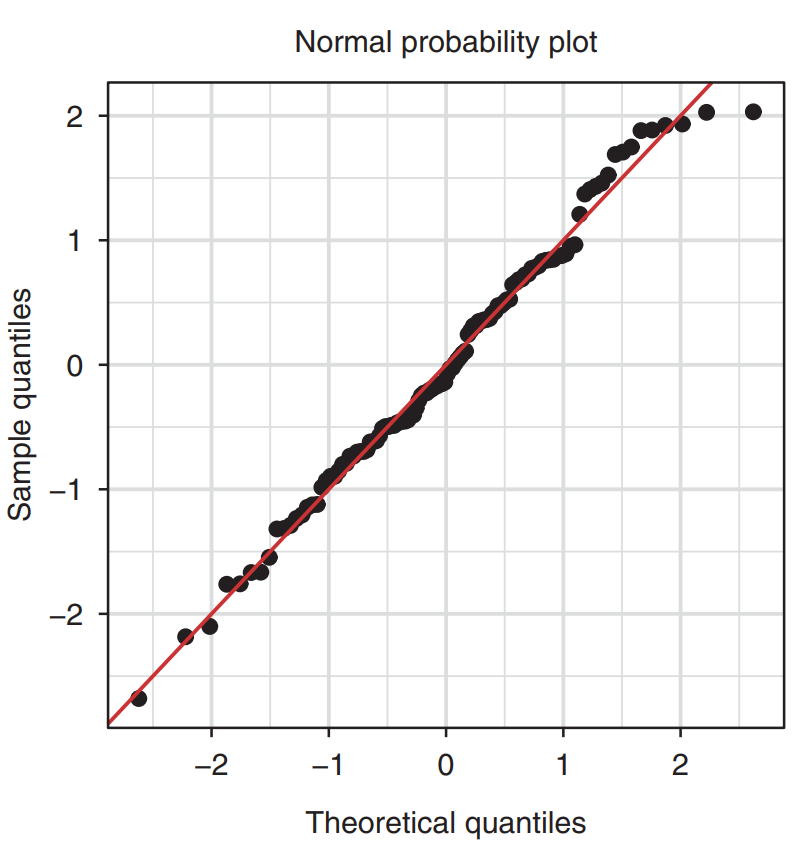
\includegraphics[scale=0.4]{gambar/plotregresilinear.png}
  \caption{Contoh plot untuk regresi linear (Rivera, 2020).}
  \label{fig:plotregresilinear}
\end{figure}

Regresi linier melayani tiga tujuan utama: menggambarkan fenomena data, kontrol, dan prediksi. Pertama, analisis regresi memungkinkan deskripsi fenomena data dengan membuat model hubungan numerik. Model ini membantu untuk memahami pola dan hubungan yang mendasari data yang sedang dipelajari.Kedua, regresi dapat digunakan untuk tujuan kontrol. Dengan menggunakan model regresi yang diperoleh, dimungkinkan untuk mengontrol atau memanipulasi variabel independen untuk melihat pengaruhnya terhadap variabel dependen. Hal ini memungkinkan untuk mempelajari hubungan sebab-akibat dan menentukan pengaruh variabel tertentu pada hasil yang diinginkan.Terakhir, analisis regresi memfasilitasi prediksi. Model regresi dapat digunakan untuk membuat prediksi terhadap variabel dependen. Namun, penting untuk dicatat bahwa prediksi terbatas pada kisaran variabel independen yang digunakan dalam membangun model regresi. Misalnya, jika model regresi dibangun menggunakan data variabel independen yang berkisar antara 5 hingga 25, prediksi hanya dapat dilakukan dalam rentang tersebut. Konsep ini dikenal sebagai interpolasi, di mana prediksi dibuat untuk nilai-nilai dalam rentang variabel independen yang diamati (Sulardi et al., 2017).

Dalam regresi linier, variabel bebas X dapat didasarkan pada data pengamatan atau data eksperimen/tetap. Data observasi mengacu pada data yang tidak ditentukan sebelumnya oleh peneliti dan diperoleh melalui observasi di lapangan. Di sisi lain, data eksperimen atau tetap mengacu pada data yang telah dikontrol atau ditentukan oleh peneliti sebelumnya, biasanya melalui eksperimen laboratorium.Perbedaan utama antara kedua jenis data ini terletak pada tingkat kontrol dan kemampuan untuk membangun hubungan sebab akibat. Saat menggunakan data tetap, peneliti memiliki nilai yang telah ditentukan sebelumnya untuk variabel independen X yang ingin mereka selidiki. Ini memungkinkan pengaturan yang lebih terkontrol dan memungkinkan peneliti untuk membangun hubungan kausal yang lebih kuat antara variabel X dan variabel dependen Y. Sebaliknya, data observasi tidak serta merta membangun hubungan sebab akibat. Variabel X dalam data observasi dapat diamati dengan berbagai cara, tergantung pada situasi nyata di lapangan. Data observasi sering dikumpulkan melalui kuesioner atau survei, dan peneliti kurang memiliki kendali atas variabel yang diteliti.


\subsection{Regresi Polinomial}
\label{subsec:regresipolinomial}

Regresi polinomial adalah teknik statistik yang memungkinkan pemodelan hubungan antara beberapa variabel independen (X dan Y) dan variabel dependen (Z) melalui hubungan non-linear (Shanock et al., 2010). Prosesnya melibatkan analisis hierarki persamaan polinomial, dengan memasukkan suku-suku orde tinggi sampai varians yang dijelaskan oleh persamaan orde tinggi berikutnya tidak lagi signifikan secara statistik. Awalnya, skor komponen untuk X dan Y (direpresentasikan sebagai X1 dan Y1) digunakan untuk menguji hubungan liniernya dengan Z pada tahap pertama analisis. Pada tahap kedua, suku orde tinggi (X2 dan Y2) dimasukkan ke dalam persamaan bersama dengan suku hasil kali (XY) untuk menilai keberadaan hubungan lengkung (khususnya, kuadrat). Selain itu, regresi polinomial, dikombinasikan dengan metodologi permukaan respons, menawarkan kerangka kerja untuk menguji dan menginterpretasikan fitur permukaan yang sesuai dengan persamaan regresi kuadrat polinomial. Teknik-teknik ini umumnya digunakan dalam penelitian organisasi, baik di tingkat mikro maupun makro, untuk menguji kesesuaian dan/atau perbedaan antar variabel (Shanock et al., 2010).

Metodologi ini memungkinkan peneliti untuk mengeksplorasi bagaimana kombinasi dua variabel prediktor dikaitkan dengan variabel hasil. Mereka telah menemukan aplikasi yang luas dalam penelitian umpan balik multi-sumber (Shanock et al., 2010). Kombinasi dari teknik-teknik ini menawarkan alat statistik yang memungkinkan pemeriksaan mendalam tentang hubungan tripartit. Dengan menyelidiki variabel dalam ruang tiga dimensi, ini memberikan wawasan tentang hubungan antara kombinasi dua variabel prediktor dan variabel hasil (Shanock et al., 2010).

Regresi polinomial dan metodologi permukaan respons dapat diterapkan dalam skenario di mana penyelidikan berfokus pada bagaimana kombinasi dua variabel prediktor berhubungan dengan suatu hasil. Namun, asumsi tertentu harus dipenuhi untuk menggunakan teknik ini secara efektif. Pertama, variabel prediktor harus sepadan, mewakili domain konseptual yang sama dan memungkinkan interpretasi yang berarti dari hubungannya dengan variabel dependen. Kedua, jika skala variabel prediktor berbeda, mereka harus diubah atau distandarisasi menjadi metrik umum. Ketiga, asumsi standar yang terkait dengan regresi berganda perlu dipenuhi (Sedera et al., 2019). Regresi polinomial dapat digunakan sebagai alternatif regresi moderat untuk memeriksa hubungan antara kombinasi variabel, menawarkan kekuatan penjelas yang lebih besar dan pandangan bernuansa dalam ruang tiga dimensi. Selanjutnya, teknik ini cocok ketika asumsi teoretis yang mendasari menunjukkan hubungan non-linear antara variabel independen dan dependen. Setelah asumsi terpenuhi, regresi polinomial dilakukan untuk menyelesaikan persamaan polinomial dan mendapatkan output. Keluaran ini kemudian dapat diproyeksikan ke permukaan respons tiga dimensi. Panduan langkah demi langkah terperinci untuk melakukan regresi polinomial dan membuat permukaan respons menggunakan keluaran polinomial disediakan oleh Shanock et al. (Shanock et al., 2010).

Pada Gambar 1, Panel A menampilkan sumbu X, Y, dan Z bersama dengan garis kongruensi dan inkongruensi. Di sisi lain, Panel B menunjukkan grafik permukaan respons sampel yang menampilkan dua variabel prediktor (X dan Y) dan satu variabel dependen (Z) (Sedera et al., 2019).

\begin{figure}[H]
  \centering
  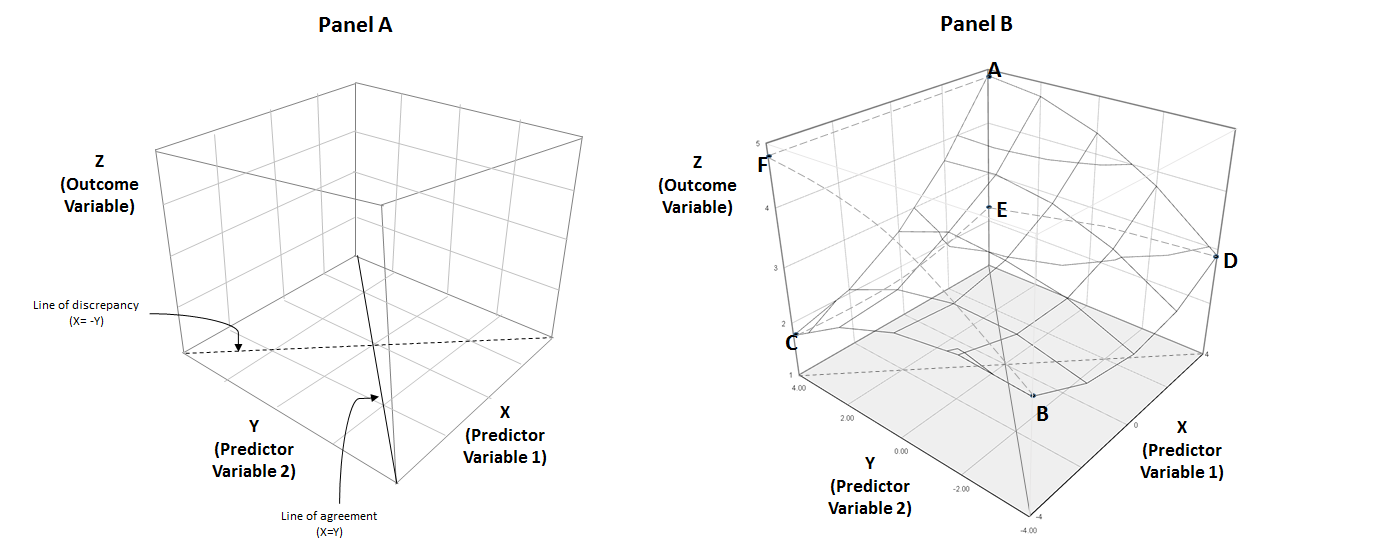
\includegraphics[scale=1]{gambar/plotregresipoli.png}
  \caption{Contoh plot untuk regresi polinomial pada 3D (Sedera et al., 2019).}
  \label{fig:plotregresipoli}
\end{figure}

\section{\emph{Machine Learning}}
\label{sec:machinelearning}

\emph{Machine Learning} (ML) adalah cabang ilmu komputasi yang muncul dari studi klasifikasi data dan prinsip-prinsip \emph{Artificial Intelligence} (AI). Bidang ini melibatkan pelatihan komputer untuk belajar secara otomatis dari input data, tanpa perlu pemrograman eksplisit. Konsep pembelajaran dalam pembelajaran mesin menarik kesejajaran dari pembelajaran manusia dan hewan. Faktanya, banyak teknik pembelajaran mesin terinspirasi oleh model komputasi berdasarkan prinsip pembelajaran hewan dan manusia. Misalnya, pembiasaan adalah perilaku kognitif mendasar yang diamati pada hewan, di mana mereka secara bertahap berhenti merespons rangsangan berulang. Anjing, misalnya, berfungsi sebagai contoh utama pembelajaran hewan, karena mereka dapat menjalani pelatihan substansial untuk melakukan berbagai aktivitas seperti berguling, duduk, dan mengambil objek (Datta \& Davim, 2022).

\begin{figure}[H]
  \centering
  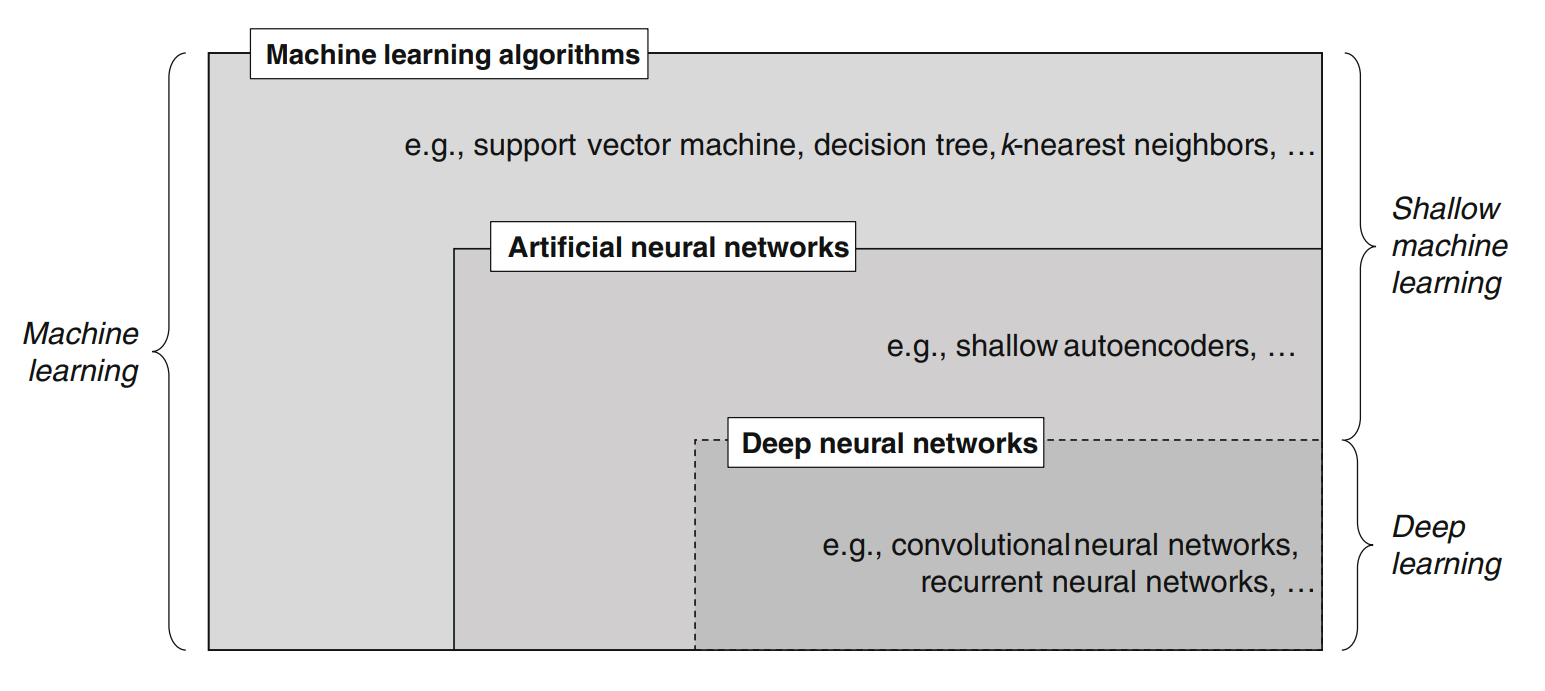
\includegraphics[scale=0.3]{gambar/machinelearning.png}
  \caption{Diagram Venn konsep dan kelas \emph{machine learning} (Janiesch et al., 2021).}
  \label{fig:machinelearningdiagram}
\end{figure}

Pembelajaran mesin menemukan aplikasi praktis dalam berbagai aspek kehidupan kita sehari-hari di era modern. Misalnya, asisten pribadi virtual, seperti Siri atau Alexa, menggunakan teknik pembelajaran mesin untuk memahami dan merespons perintah pengguna. Sistem navigasi GPS memanfaatkan pembelajaran mesin untuk memprediksi kondisi lalu lintas dan menyarankan rute yang optimal. Sistem pengawasan bertenaga AI dapat menganalisis umpan dari beberapa kamera untuk mendeteksi potensi kejahatan atau perilaku yang tidak biasa. Platform media sosial memanfaatkan pembelajaran mesin untuk tugas-tugas seperti pengenalan wajah dan kurasi umpan berita yang dipersonalisasi. Mesin pencari terus menyempurnakan hasil mereka menggunakan algoritma pembelajaran mesin. Filter spam email belajar dari email spam berlabel sebelumnya untuk mengidentifikasi dan memblokir pesan yang tidak diinginkan. Ini hanyalah beberapa contoh yang menunjukkan penggunaan luas pembelajaran mesin dalam aplikasi praktis. Memasukkan pengetahuan sebelumnya ke dalam proses pembelajaran dapat secara signifikan meningkatkan keefektifannya. Pembelajaran mesin juga terkait erat dengan statistik komputasi, memungkinkan pemodelan prediktif. Pentingnya pembelajaran mesin terletak pada pemahaman bagaimana hewan dan manusia belajar, serta dalam berbagai tujuan praktisnya (Datta \& Davim, 2022).

\subsection{\emph{Supervised Learning}}
\label{subsec:supervisedlearning}

Pembelajaran yang diawasi melibatkan penggunaan kumpulan data pelatihan yang berisi contoh dengan data input dan nilai target berlabel. Misalnya, memprediksi jumlah pengguna aktif pada platform pasar di bulan mendatang dapat dianggap sebagai tugas pembelajaran yang diawasi. Dalam hal ini, fitur input, seperti jumlah produk yang terjual atau review pengguna yang positif, digunakan untuk memprediksi variabel target atau output (sering dinotasikan sebagai variabel "y"). Dataset pelatihan digunakan untuk menyesuaikan parameter model pembelajaran mesin. Setelah model berhasil dilatih, model tersebut dapat diterapkan untuk memprediksi variabel target untuk titik data baru atau yang tidak terlihat berdasarkan fitur inputnya. Pembelajaran yang diawasi dapat dikategorikan lebih lanjut ke dalam masalah regresi, di mana nilai numerik diprediksi (mis., Jumlah pengguna), dan masalah klasifikasi, di mana hasil prediksi mewakili label kelas kategori, seperti "penonton" atau "pembeli" (Janiesch et al., 2021).

\subsection{\emph{Unsupervised Learning}}
\label{subsec:unsupervisedlearning}

Pembelajaran tanpa pengawasan terjadi ketika sistem pembelajaran ditugaskan untuk mengidentifikasi pola dalam data tanpa label atau spesifikasi yang telah ditentukan sebelumnya. Dalam pembelajaran tanpa pengawasan, data pelatihan hanya terdiri dari variabel (dilambangkan sebagai "x"), yang bertujuan untuk menemukan informasi struktural yang bermakna. Ini dapat melibatkan pendeteksian kelompok elemen yang memiliki sifat umum, yang dikenal sebagai pengelompokan, atau pengurangan dimensi data dengan memproyeksikannya dari ruang dimensi yang lebih tinggi ke ruang dimensi yang lebih rendah, yang dikenal sebagai pengurangan dimensi. Dalam konteks pasar elektronik, contoh menonjol dari pembelajaran tanpa pengawasan adalah penerapan teknik pengelompokan untuk mengelompokkan pelanggan atau pasar ke dalam segmen-segmen. Ini memungkinkan komunikasi yang lebih bertarget dan spesifik yang disesuaikan dengan kelompok pelanggan yang berbeda (Janiesch et al., 2021).

\subsection{\emph{Semi Supervised Learning}}
\label{subsec:semiisupervisedlearning}

Pembelajaran semi-diawasi adalah pendekatan hybrid yang menggabungkan metode pembelajaran yang diawasi dan tidak diawasi, dengan fokus pada penggunaan sampel berlabel dan tidak berlabel secara efektif selama proses pelatihan. Ini bertujuan untuk membangun hubungan antara sampel yang diprediksi dan tujuan pembelajaran berdasarkan hipotesis tertentu. Asumsi kehalusan menunjukkan bahwa sampel yang terletak berdekatan di wilayah kepadatan tinggi lebih cenderung memiliki label kelas yang sama. Asumsi cluster berpendapat bahwa sampel yang termasuk dalam cluster yang sama sangat mungkin untuk berbagi kelas yang sama. Terakhir, asumsi manifold mengusulkan bahwa sampel dalam lingkungan lokal kecil dalam manifold berdimensi rendah cenderung memiliki label kelas yang serupa (Wang et al., 2023).

\subsection{\emph{Reinforcement Learning}}
\label{subsec:reinforcementlearning}

Dalam sistem pembelajaran penguatan, pendekatannya berbeda dengan pemberian pasangan input-output. Sebaliknya, sistem dijelaskan oleh keadaan saat ini, tujuan yang ditentukan, serangkaian tindakan yang diizinkan, dan kendala lingkungan terkait untuk setiap hasil tindakan. Model pembelajaran mesin kemudian belajar dengan secara aktif terlibat dalam proses pencapaian tujuan melalui coba-coba, yang bertujuan untuk memaksimalkan hadiah. Pembelajaran penguatan telah menunjukkan pencapaian yang signifikan dalam lingkungan yang terkendali seperti permainan dan juga berlaku untuk sistem multi-agen seperti pasar elektronik (Janiesch et al., 2021).

\section{\emph{Deep Learning}}
\label{sec:deeplearning}

\emph{Deep learning} adalah cabang \emph{machine learning} yang melibatkan penggunaan beberapa lapisan pemrosesan informasi nonlinier untuk melakukan tugas-tugas seperti ekstraksi fitur, pengenalan pola, dan klasifikasi (Deng dan Yu, 2014). Menurut Goodfellow, dkk. (2016) dalam \emph{deep learning}, konsep kompleks dipelajari dengan menggabungkan konsep yang lebih sederhana secara hierarkis. Struktur hierarkis ini memungkinkan komputer mempelajari dan memahami pola dan hubungan yang rumit di dalam data. Istilah "dalam" mengacu pada beberapa lapisan dalam jaringan, membentuk grafik yang dalam saat divisualisasikan, oleh karena itu dinamakan "pembelajaran mendalam". \emph{Deep learning} telah terbukti sangat efektif di berbagai bidang, termasuk visi komputer, pemrosesan bahasa alami, dan pengenalan suara.

\emph{Deep learning} dicirikan oleh arsitekturnya yang terdiri dari beberapa lapisan, umumnya dikenal sebagai \emph{hidden layer}, yang ditumpuk bersama. Setiap lapisan dalam arsitektur ini berfungsi sebagai algoritma atau metode yang mengambil input dan menghasilkan output melalui serangkaian komputasi. Salah satu metode \emph{deep learning} yang menonjol adalah \emph{Convolutional Neural Network} (CNN). CNN dirancang khusus untuk memproses input gambar. Gambar input melewati lapisan konvolusional, di mana diproses menggunakan filter yang mengekstraksi pola dari berbagai bagian gambar. Ekstraksi pola hierarkis dari gambar ini membantu dalam proses klasifikasi. CNN telah menunjukkan keberhasilan luar biasa dalam berbagai tugas terkait gambar seperti pengenalan objek, klasifikasi gambar, dan segmentasi gambar (Danukusumo, 2017).

\begin{figure}[H]
  \centering
  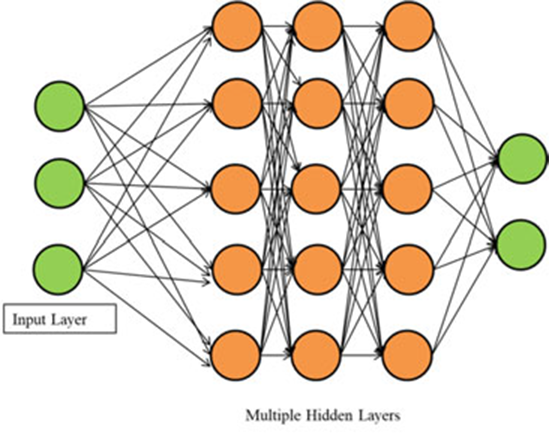
\includegraphics[scale=1]{gambar/arsitekturdlnn.png}
  \caption{Arsitektur \emph{deep learning} (Janiesch et al., 2021)}
  \label{fig:arsidl}
\end{figure}


Di bidang pengenalan citra, \emph{Convolutional Neural Network} (CNN) saat ini merupakan metode \emph{deep learning} yang paling berdampak (Nugroho et al., 2020). CNN sangat berhasil dalam lingkup ini karena mencoba meniru sistem pengenalan gambar dari korteks visual manusia, memungkinkannya memproses informasi gambar secara efektif. Namun, seperti metode pembelajaran mendalam lainnya, CNN memiliki kekurangan, yaitu proses pelatihan yang lama. Untungnya, kemajuan teknologi perangkat keras, seperti penggunaan \emph{General Purpose Graphical Processing Unit} (GPGPU), telah membantu mengatasi tantangan ini.

CNN dirancang dengan fokus khusus pada tugas yang terkait dengan pengenalan dan klasifikasi gambar. Arsitektur dan strukturnya disesuaikan untuk memproses dan menganalisis data gambar secara efisien. Ini terdiri dari beberapa lapisan yang mengekstrak informasi yang relevan dari gambar dan membuat prediksi tentang klasifikasinya melalui skor klasifikasi. Lapisan di CNN, seperti lapisan konvolusional dan lapisan penyatuan, memainkan peran penting dalam menangkap fitur dan pola hierarki dalam gambar, memungkinkan pengenalan dan klasifikasi yang akurat. Secara keseluruhan, kemampuan CNN untuk mempelajari dan menginterpretasikan data visual yang kompleks menjadikannya metode terdepan dalam bidang pengenalan gambar.

\subsection{\emph{Neural Network}}
\label{subsec:cnn}

Artificial Neural Networks (ANNs) adalah sistem komputasi yang mengambil inspirasi dari Biological Neural Networks (BNNs). Mereka menawarkan solusi yang efektif untuk berbagai tugas, seperti klasifikasi, prediksi, pemfilteran, pengoptimalan, pengenalan pola, dan perkiraan fungsi. Sementara sistem saraf biologis sangat rumit, JST bertujuan untuk menyederhanakan dan abstrak kompleksitas ini, berfokus pada aspek-aspek penting yang relevan dengan pemrosesan informasi. Jaringan saraf awalnya diperkenalkan oleh McCulloch dan Pitts pada tahun 1990 ketika mereka berusaha memodelkan pemrosesan informasi secara matematis dalam sistem biologis. Jaringan ini terdiri dari simpul yang saling berhubungan, menyerupai neuron yang ditemukan di otak organisme hidup. Setiap node menghitung jumlah bobot inputnya, memprosesnya di dalam lapisan tersembunyi, dan menghasilkan output dengan menerapkan fungsi aktivasi ke nilai bobot (Thakur et al., 2021).

\begin{figure}[H]
  \centering
  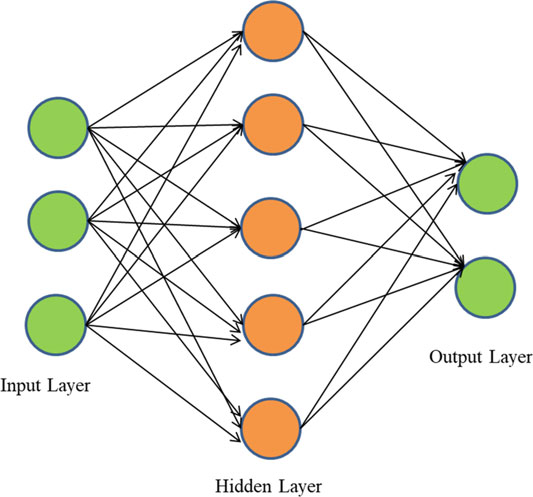
\includegraphics[scale=1]{gambar/arsitekturann.png}
  \caption{Arsitektur \emph{neural network} (Janiesch et al., 2021)}
  \label{fig:arsiann}
\end{figure}

Neural network telah berevolusi dari arsitektur sederhana menjadi struktur yang semakin kompleks. Awalnya, jaringan saraf memiliki arsitektur yang sangat dasar yang hanya terdiri dari lapisan masukan dan keluaran, sering disebut sebagai jaringan lapisan tunggal. Namun, dengan memasukkan lapisan tersembunyi ke dalam jaringan saraf satu lapis, itu menjadi jaringan saraf multi-lapisan. Akibatnya, jaringan saraf multi-layer terdiri dari lapisan input, lapisan tersembunyi, dan lapisan output, seperti yang diilustrasikan pada gambar yang diberikan (Thakur et al., 2021).

\section{\emph{Convolutional Neural Network}}
\label{sec:cnn}

\emph{Convolutional Neural Network} (CNN) adalah jenis jaringan saraf khusus yang biasa digunakan dalam tugas pemrosesan gambar untuk mendeteksi dan mengenali objek di dalam gambar (Mehindra, 2020). CNN dirancang untuk memproses data yang diatur dalam struktur seperti kisi, seperti gambar. Mereka dapat dianggap sebagai kombinasi jaringan syaraf tiruan dan metode pembelajaran mendalam (Fonda, 2020). Arsitektur CNN tipikal terdiri dari satu atau lebih lapisan konvolusional, yang melakukan konvolusi pada data input, diikuti oleh lapisan downsampling, sering disebut sebagai lapisan penyatuan. Lapisan-lapisan ini membantu mengurangi dimensi spasial data sambil mempertahankan fitur-fitur penting. Terakhir, satu atau lebih lapisan yang terhubung sepenuhnya digabungkan, mirip dengan jaringan saraf tradisional, untuk memproses fitur yang diekstraksi dan membuat prediksi. Dengan menggunakan lapisan konvolusional, CNN efektif dalam menangkap ketergantungan spasial dan lokal dalam gambar, memungkinkan mereka untuk mempelajari representasi dan pola yang bermakna. Ini membuat CNN sangat cocok untuk tugas-tugas seperti klasifikasi gambar, deteksi objek, dan segmentasi gambar.

Arsitektur CNN dapat dibagi menjadi dua bagian utama, yaitu \emph{Fully-Connected Layer} dan \emph{Multi-Layer Perceptron} (MLP). CNN terdiri dari beberapa lapisan yang melakukan operasi tertentu. Mengikuti arsitektur LeNet5, terdapat empat layer utama dalam sebuah CNN berupa \emph{Convolution Layer, Pooling Layer, Subsampling Layer,} dan \emph{Fully Connected Layer} (Eka Putra, 2016). 

\begin{figure}[H]
  \centering
  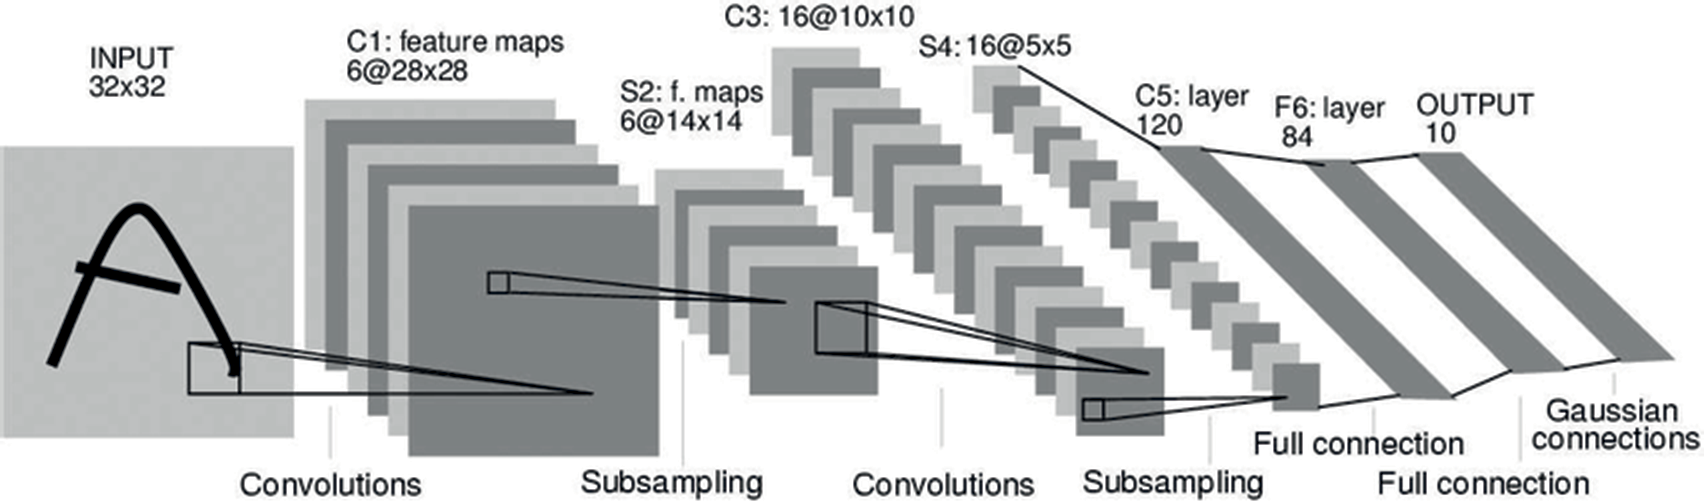
\includegraphics[scale=0.8]{gambar/arsitekturcnn.png}
  \caption{Arsitektur \emph{convolutional neural network} oleh LeNet-5 (LeCun et al., 1998)}
  \label{fig:arsicnn}
\end{figure}

\emph{Convolution Layer} menerapkan operasi konvolusi untuk mengekstraksi fitur dari data masukan. Ini menggunakan filter untuk mendeteksi berbagai pola dan struktur dalam data. \emph{Pooling layer} mengurangi dimensi spasial dari fitur yang diekstraksi sambil mempertahankan karakteristik pentingnya. Ini membantu mengurangi kompleksitas komputasi dan membuat jaringan lebih kuat terhadap variasi dalam input data. \emph{Subsampling layer} selanjutnya mengurangi dimensi data melalui \emph{downsampling}, menangkap informasi yang paling signifikan. Terakhir, \emph{Fully-Connected Layer}, yang serupa dengan \emph{Multi-Layer Perceptron} (MLP), menerima fitur yang diproses dan melakukan tugas klasifikasi atau regresi. Ini menghubungkan semua neuron dari lapisan sebelumnya ke lapisan keluaran, memungkinkan jaringan membuat prediksi berdasarkan fitur yang dipelajari. Lapisan-lapisan ini bekerja sama dalam CNN untuk mengekstraksi dan mengubah data input menjadi representasi yang bermakna, yang pada akhirnya memungkinkan jaringan untuk melakukan tugas-tugas seperti pengenalan gambar dan klasifikasi secara efektif.

Pada CNN, data yang diproses oleh jaringan berupa data dua dimensi. Ini memerlukan adaptasi khusus dalam hal operasi linier dan bobot parameter di CNN dibandingkan dengan jaringan saraf tradisional. CNN menggunakan operasi konvolusi untuk operasi linier, dan bobot direpresentasikan dalam empat dimensi sebagai sekumpulan kernel konvolusi. Karena sifat yang melekat pada proses konvolusi, CNN cocok untuk menganalisis data dengan struktur dua dimensi, seperti gambar dan suara.

Sebagai contoh adalah data yang diproses CNN berupa gambar dua dimensi. Istilah "konvolusi" mengacu pada operasi aljabar linier di mana matriks filter dikalikan dengan matriks gambar yang sedang diproses. Operasi ini dikenal sebagai lapisan konvolusi, yang merupakan salah satu dari beberapa jenis lapisan yang dapat hadir dalam CNN. Lapisan konvolusi sangat penting dan banyak digunakan dalam arsitektur CNN. Lapisan lain yang umum digunakan adalah \emph{Pooling layer}, yang mengagregasi informasi dengan mengambil nilai maksimum atau rata-rata dari wilayah piksel di dalam gambar. Setiap lapisan masukan dalam CNN memiliki volume berbeda yang ditandai dengan kedalaman, tinggi, dan lebarnya. Nilai yang didapat pada setiap layer dipengaruhi oleh hasil proses penyaringan dari layer sebelumnya, serta jumlah filter yang digunakan. Model jaringan ini telah menunjukkan kemanjuran yang luar biasa dalam menangani tugas klasifikasi gambar.

\subsection{\emph{Convolutional Layer}}
\label{subsec:cnn}

Operasi konvolusi adalah komponen fundamental dari jaringan saraf convolutional (CNN). Lapisan convolutional dari CNN terdiri dari satu set filter yang dapat dipelajari, juga dikenal sebagai kernel. Setiap filter berukuran kecil, biasanya 3x3, 5x5, atau 7x7, dan menjangkau seluruh kedalaman volume input. Kedalaman filter sesuai dengan jumlah saluran dalam masukan, dengan gambar skala abu-abu memiliki kedalaman 1 dan gambar berwarna memiliki 3 saluran (RGB) (Bezdan et al., 2019). 

Selama proses propagasi maju dalam jaringan saraf convolutional, setiap filter melakukan konvolusi pada volume input dengan menghitung perkalian titik antara entri filter dan nilai input yang sesuai di setiap posisi. Operasi ini diikuti dengan menerapkan fungsi aktivasi nonlinier, seperti sigmoid, tanh, atau ReLU, ke hasilnya, yang menghasilkan peta fitur. Peta fitur mewakili respons filter pada posisi spasial yang berbeda. Peta aktivasi ini ditumpuk sepanjang dimensi kedalaman untuk membentuk volume keluaran. Karakteristik volume output ditentukan oleh tiga hyperparameter: depth, stride, dan padding (Bezdan et al., 2019).

Kedalaman volume keluaran sesuai dengan jumlah filter yang digunakan dalam operasi konvolusi. Setiap filter mempelajari aspek input yang berbeda, seperti tepi, blob, atau warna. Langkahnya menentukan jumlah langkah filter bergerak melintasi input. Langkah 1 menggerakkan filter satu piksel pada satu waktu, sedangkan langkah 2 membuat filter melompati 2 piksel sekaligus, menghasilkan volume output yang lebih kecil secara spasial. Padding digunakan untuk mengontrol ukuran output. Ini melibatkan penambahan nol di sekitar batas volume input untuk menyimpan informasi dan menghindari pengurangan ukuran output. Ada dua pilihan umum: valid convolution, yang berarti tidak ada padding, dan same convolution, di mana ukuran output tetap sama dengan ukuran input (Bezdan et al., 2019).

\subsection{\emph{Pooling Layer}}
\label{subsec:cnn}

Pooling layer di CNN sering digunakan setelah convolutional layer untuk mengurangi dimensi peta fitur. Operasi ini juga dikenal sebagai subsampling atau downsampling. Hyperparameters dari pooling layer mencakup ukuran dan langkah filter. Lapisan penyatuan yang paling umum digunakan memiliki ukuran filter 2 dan langkah 2. Ada dua jenis utama penyatuan lapisan: penyatuan maks dan penyatuan rata-rata. Max pooling memilih nilai maksimum dalam setiap wilayah, sedangkan average pooling menghitung nilai rata-rata. Max pooling lebih umum digunakan daripada pooling rata-rata. Penting untuk diperhatikan bahwa pooling layer tidak memiliki parameter yang dapat dipelajari. Tujuan max pooling adalah untuk menangkap fitur yang paling menonjol dengan memilih nilai terbesar (Bezdan et al., 2019).


\subsection{\emph{Fully Connected Layer}}
\label{subsec:cnn}

Setelah beberapa lapisan konvolusi dan penyatuan, CNN biasanya diakhiri dengan beberapa lapisan yang terhubung sepenuhnya. Output tensor dari lapisan sebelumnya diratakan menjadi vektor, dan kemudian ditambahkan lapisan jaringan saraf tambahan. Lapisan yang terhubung penuh ini biasanya diposisikan menjelang akhir arsitektur, seperti yang digambarkan pada Gambar 3. Untuk mencegah overfitting, teknik regularisasi dropout dapat digunakan pada lapisan yang terhubung penuh ini. Lapisan terhubung penuh terakhir dalam arsitektur terdiri dari jumlah neuron keluaran yang sama dengan jumlah kelas yang akan dikenali (Bezdan et al., 2019).

\section{Visi Komputer}
\label{sec:deteksigesturtubuh}

Visi komputer adalah bidang kecerdasan buatan yang bertujuan untuk meniru persepsi visual manusia dengan menggunakan algoritme dan sensor optik untuk mengekstrak informasi yang relevan dari objek. Tidak seperti metode tradisional yang melibatkan pemeriksaan laboratorium yang memakan waktu dan tenaga, visi komputer menawarkan pendekatan yang lebih efisien. Integrasi sistem pencahayaan dapat digunakan bersamaan dengan MediaPipe untuk meningkatkan proses akuisisi dan pemrosesan gambar. Proses analisis citra melibatkan beberapa langkah. Pertama, tahap pembentukan citra menangkap dan menyimpan citra suatu objek di dalam komputer. Selanjutnya, pra-pemrosesan gambar meningkatkan kualitas gambar untuk meningkatkan detail. Kemudian, segmentasi citra mengidentifikasi dan memisahkan citra objek dari latar belakang. Pada tahap pengukuran citra dilakukan pengukuran berbagai parameter penting. Akhirnya, interpretasi gambar melibatkan analisis dan pemahaman gambar yang diperoleh (Kotappa  et al., 2022).

\begin{figure}[H]
  \centering
  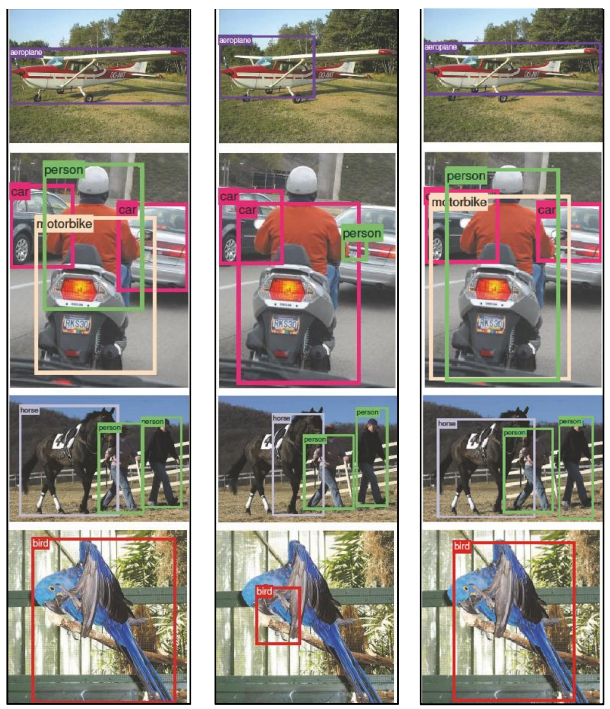
\includegraphics[scale=0.55]{gambar/computervision.png}
  \caption{Visi komputer pada deteksi objek (Shetty et al., 2022)}
  \label{fig:visikomdeteksi}
\end{figure}

Karena kemajuan terbaru dalam teknologi pemrosesan gambar, sekarang dimungkinkan untuk mengembangkan sistem yang dapat mengenali gambar digital. Bidang-bidang seperti matematika, aljabar linier, statistik, Soft Computing, dan ilmu saraf Komputasi telah memainkan peran penting dalam memajukan pemrosesan citra digital. Pengenalan pola, bagian dari visi komputer, berfokus pada identifikasi objek dengan meningkatkan kualitas gambar dan interpretasi melalui transformasi gambar. Ini melibatkan penggalian data dari gambar yang ditangkap sensor untuk membuat penilaian. Tujuan dari visi komputer adalah menciptakan mesin yang dapat "melihat". Kerangka umum dalam visi komputer mencakup pengambilan gambar, pemrosesan awal, ekstraksi fitur, deteksi/segmentasi, pemrosesan tingkat tinggi, dan pengambilan keputusan. Dalam visi komputer, ada kategori seperti analisis morfologi 3D dan pengoptimalan piksel. Optimalisasi piksel melibatkan karakterisasi morfologi piksel untuk pemrosesan gambar yang lebih baik dan pengenalan pola, sedangkan analisis morfologi 3D adalah teori standar dalam pemrosesan gambar komputer dan pengenalan pola (Kotappa  et al., 2022).

Kategori ini mencakup tugas-tugas yang terkait dengan pengambilan wilayah gambar tertentu, seperti kueri mesin telusur, penelusuran manusia, dan penelusuran gambar serupa. Metode segmentasi gambar, seperti pendekatan berbasis intensitas, berbasis warna, dan berbasis bentuk, biasanya digunakan untuk tujuan ini. Deteksi tepi dan segmentasi gambar sangat penting untuk pengenalan dan interpretasi objek dalam berbagai aplikasi visi komputer. Sementara gambar sampel kecil sering digunakan untuk mendemonstrasikan kinerja segmentasi dalam literatur analisis gambar, pengaturan parameter diperlukan untuk anotasi dalam database gambar berskala besar. Tekstur gradien dan pengelompokan tanpa pengawasan dalam ruang fitur digunakan untuk mencapai segmentasi. Segmentasi pelabelan yang akurat sangat penting untuk kinerja pelokalan dan pelokalan batas. Pendekatan pengelompokan dan segmentasi dapat digunakan untuk memperkirakan item dalam citra dengan menetapkan ambang batas pada metode pengelompokan fitur (Kotappa  et al., 2022).


\section{Treadmill}
\label{sec:deteksigesturtubuh}

Treadmill umumnya digunakan di bidang rehabilitasi untuk membantu pasien dengan gangguan gaya berjalan, seperti penyakit Parkinson, stroke, dan cedera tulang belakang, dalam pemulihan kemampuan berjalan mereka. Pelatihan treadmill menawarkan beberapa keuntungan dibandingkan dengan pelatihan di lapangan, antara lain bantuan yang dapat diakses, kebutuhan ruang yang lebih kecil, dan kemampuan untuk mengontrol kecepatan berjalan. Namun, penting untuk dicatat bahwa tujuan akhir rehabilitasi adalah agar pasien mendapatkan kembali kemampuannya untuk berjalan di tanah daripada hanya di atas treadmill. Oleh karena itu, sangat penting untuk memahami dampak berjalan treadmill pada tubuh manusia (Shi et al., 2019).

Bidang studi ini penting untuk tujuan pelatihan dan penelitian, dan ada temuan yang bertentangan dalam studi ilmiah mengenai topik ini. Beberapa penelitian telah menunjukkan bahwa berlari di atas treadmill dengan kecepatan sedang 3,3 hingga 4,8 m/s menghasilkan penurunan panjang langkah dan fase terbang, tetapi iramanya meningkat dibandingkan dengan berlari di tanah. Di sisi lain, penelitian lain telah menemukan kesamaan antara treadmill dan lari di atas tanah dalam hal faktor kinematik seperti sudut adduksi pinggul, rotasi pinggul internal / eksternal, eversi pergelangan kaki, dan rotasi panggul maksimum (Pakbaz et al., 2018).

Belakangan ini, penggunaan perangkat treadmill meningkat secara signifikan, menjadikannya pilihan populer di kalangan individu. Selain itu, treadmill telah mendapatkan popularitas sebagai alat penelitian di berbagai bidang investigasi karena keunggulan metodologinya, termasuk efisiensi ruang, reproduktifitas, dan kemampuan untuk mengontrol variabel seperti kondisi cuaca, kecepatan, dan kemiringan. Namun, penelitian yang dilakukan pada treadmill telah menghasilkan hasil yang bertentangan, yang mengarah ke pertanyaan tentang apakah kelelahan yang disebabkan oleh berlari di atas treadmill dibandingkan berlari di tanah memiliki efek yang berbeda pada distribusi tekanan plantar selama berlari (Pakbaz et al., 2018).

\begin{figure}[H]
  \centering
  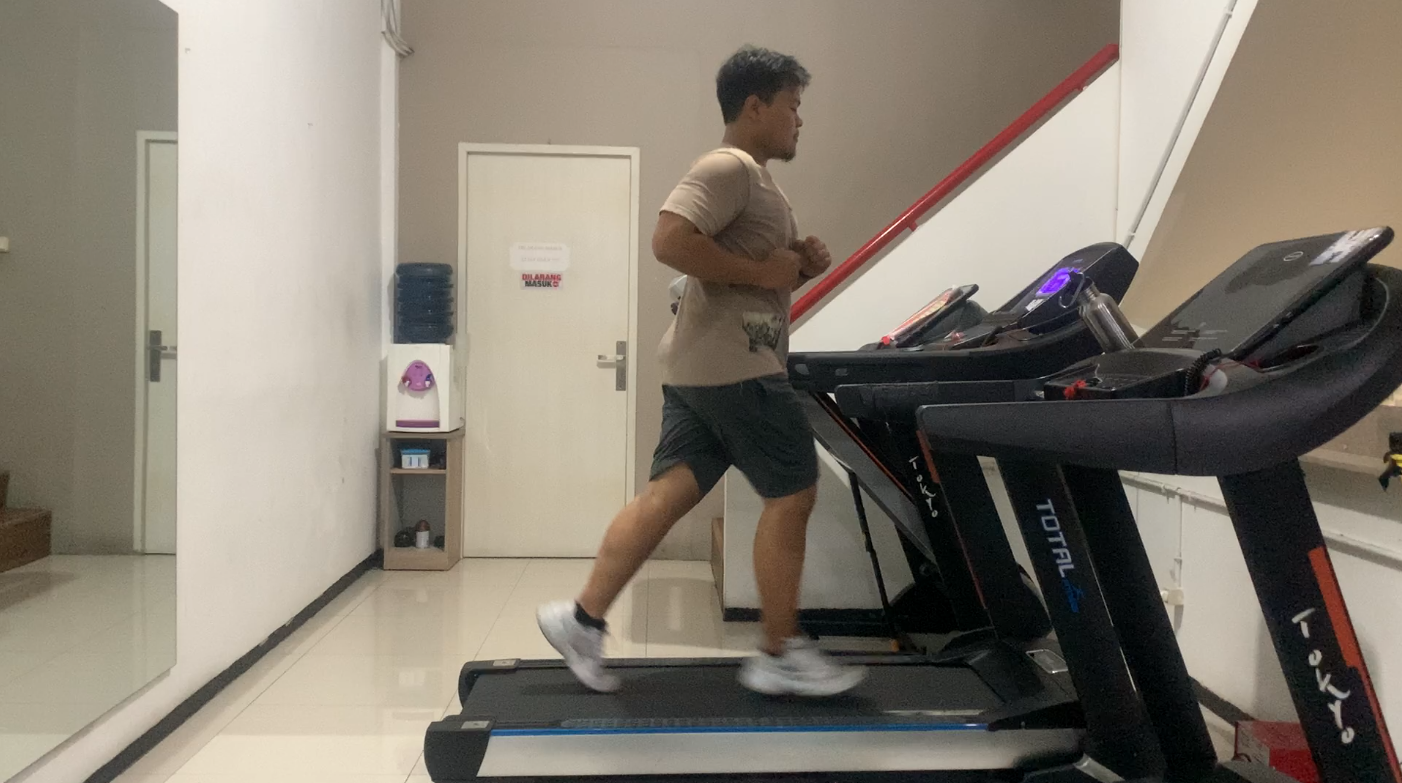
\includegraphics[scale=0.28]{gambar/treadmill.png}
  \caption{Olahraga pada treadmill.}
  \label{fig:treadmillrun}
\end{figure}

\section{\emph{Human Pose Estimation}}
\label{sec:deteksigesturtubuh}

Estimasi pose manusia bertujuan untuk menentukan posisi sendi manusia menggunakan berbagai sumber input seperti gambar, urutan gambar, gambar kedalaman, atau data kerangka yang diperoleh dari perangkat penangkap gerak. Tugas ini menantang karena faktor-faktor seperti penampilan manusia yang beragam, variasi siluet, kondisi pencahayaan yang menantang, dan latar belakang yang berantakan. Di masa lalu, estimasi pose bergantung pada teknik seperti deteksi bagian tubuh menggunakan struktur bergambar. Namun, dengan munculnya pembelajaran mendalam, ada dua pendekatan utama yang digunakan: metode holistik dan berbasis bagian (Shetty et al., 2022).

\begin{figure}[H]
  \centering
  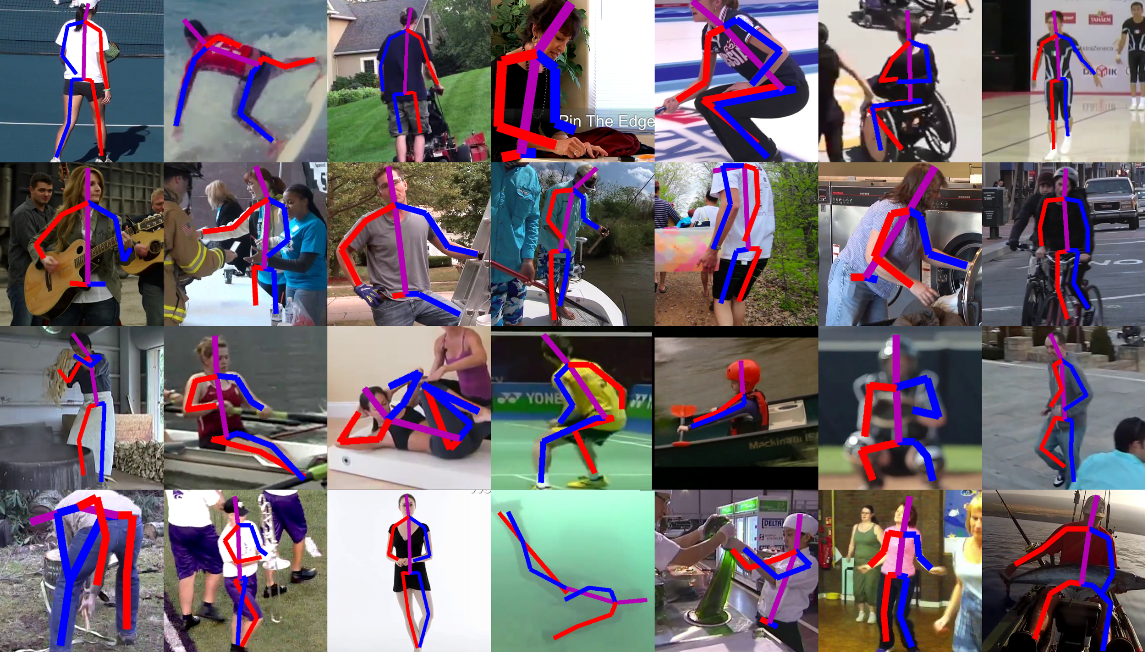
\includegraphics[scale=0.95]{gambar/humanpose.png}
  \caption{Contoh hasil \emph{human pose estimation} (Newell et al., 2016)}
  \label{fig:humanposeestimation}
\end{figure}

Metode holistik memproses gambar masukan secara global tanpa secara eksplisit memodelkan bagian tubuh individu dan hubungan spasialnya. Misalnya, DeepPose adalah model holistik yang memperlakukan estimasi pose manusia sebagai masalah regresi gabungan, tanpa secara eksplisit mendefinisikan model grafis atau pendeteksi bagian. Namun, pendekatan holistik mungkin berjuang dengan akurasi di wilayah presisi tinggi karena kesulitan untuk secara langsung meregresi vektor pose kompleks dari gambar (Shetty et al., 2022).

Di sisi lain, metode berbasis bagian secara eksplisit memodelkan bagian tubuh individu dan hubungan spasialnya. Metode ini menganalisis citra masukan dengan mempertimbangkan hubungan antara berbagai bagian tubuh manusia. Dengan memodelkan bagian-bagian secara eksplisit, pendekatan ini bertujuan untuk menangkap informasi yang lebih rinci tentang pose tersebut (Shetty et al., 2022).

Sebaliknya, metode berbasis bagian dalam estimasi pose manusia berfokus pada pendeteksian bagian tubuh individu secara terpisah dan kemudian menggunakan model grafis untuk memasukkan informasi spasial. Misalnya, dalam satu penelitian, alih-alih melatih jaringan pada seluruh gambar, penulis melatih jaringan saraf convolutional (CNN) menggunakan tambalan bagian lokal dan tambalan latar belakang untuk mempelajari probabilitas bersyarat dari kehadiran bagian dan hubungan spasial. Pendekatan lain melibatkan pelatihan beberapa CNN yang lebih kecil untuk klasifikasi bagian tubuh biner independen, diikuti oleh model spasial lemah tingkat tinggi untuk menghilangkan outlier dan memastikan konsistensi pose global. Selanjutnya,  multi-resolusi CNN dikembangkan untuk memperkirakan kemungkinan setiap bagian tubuh menggunakan peta panas, dan model grafis implisit diterapkan untuk menegakkan konsistensi sendi (Shetty et al., 2022).

\section{Mediapipe}
\label{sec:mediapipe}

MediaPipe adalah kerangka kerja yang dirancang untuk membuat jalur pipa untuk melakukan inferensi pada berbagai jenis data sensorik. Dengan menggunakan MediaPipe, dimungkinkan untuk membuat pipa yang terdiri dari komponen modular, termasuk inferensi model, algoritme pemrosesan media, dan transformasi data. Framework ini memungkinkan input data sensorik seperti audio dan video stream ke dalam pipeline, dan menghasilkan deskripsi yang dirasakan seperti lokalisasi objek dan face landmark stream sebagai outputnya (Lugaresi et al., 2019).

\begin{figure}[H]
  \centering
  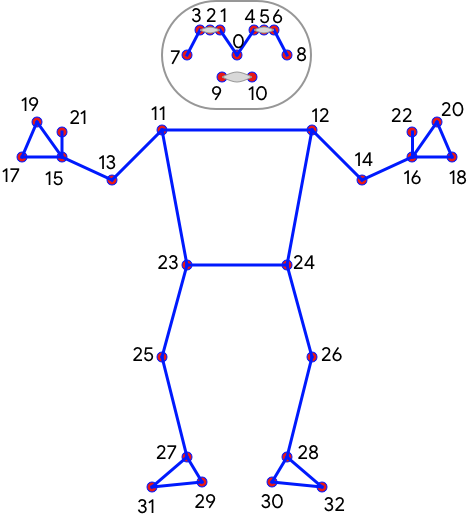
\includegraphics[scale=1.3]{gambar/mediapipeb2.png}
  \caption{Mediapipe \emph{keypoints} untuk estimasi pose (Bazarevsky et al., 2020).}
  \label{fig:mediapipe}
\end{figure}

MediaPipe adalah platform yang melayani praktisi pembelajaran mesin, termasuk peneliti, mahasiswa, dan pengembang perangkat lunak. Tujuannya adalah untuk membantu pengembangan aplikasi ML yang siap produksi, mendukung publikasi kode penelitian, dan memungkinkan pembuatan prototipe teknologi. Kasus penggunaan utama untuk MediaPipe adalah pembuatan pipeline persepsi yang cepat dan efisien dengan memanfaatkan model inferensi dan komponen yang dapat digunakan kembali. Selain itu, MediaPipe menyederhanakan penerapan teknologi persepsi dalam demonstrasi dan aplikasi di berbagai platform perangkat keras. Platform ini juga memfasilitasi peningkatan iteratif pada alur persepsi melalui bahasa konfigurasi dan alat evaluasinya yang komprehensif (Lugaresi et al., 2019).

\section{Metode Pengujian}
\label{sec:deteksigesturtubuh}

Pada metode pengujian yang dilakukan pada penelitian ini menggunakan beberapa teori dalam menentukan hasil pengujian yang digunakan. Metode pengujian yang digunakan dalam penelitian ini adalah sebagai berikut:

\subsection{\emph{Confusion Matrix}}
\label{subsec:cnn}

Metode penilaian sangat penting untuk mengevaluasi kinerja klasifikasi dan memandu pemodelan pengklasifikasi. Proses klasifikasi melibatkan tiga fase utama: pelatihan, validasi, dan pengujian. Pada fase pelatihan, model dilatih menggunakan pola masukan atau data pelatihan, dan parameter model disesuaikan. Kesalahan pelatihan mengukur seberapa cocok model dengan data pelatihan, tetapi cenderung lebih kecil daripada kesalahan pengujian dan validasi karena cocok dengan data yang sama yang digunakan dalam pelatihan. Tahap pengujian bertujuan untuk memprediksi label kelas untuk data yang tidak terlihat, tetapi kesalahan pengujian tidak dapat diperkirakan karena label kelas yang sebenarnya tidak diketahui. Di sinilah fase validasi masuk, memberikan evaluasi yang tidak bias dari model yang dilatih sambil menyetel hyperparameternya (Tharwat, 2018).

\begin{figure}[H]
  \centering
  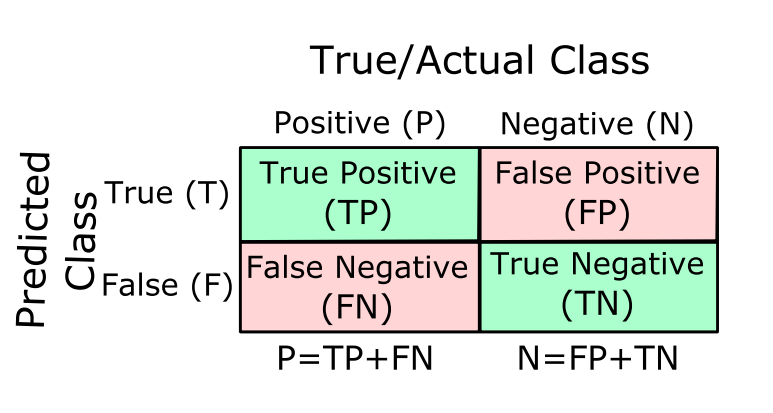
\includegraphics[scale=0.5]{gambar/confusionmatrix.png}
  \caption{Contoh \emph{Confusion Matrix} dengan dimensi 2 x 2 (Tharwat, 2018)}
  \label{fig:confusionmatrixex}
\end{figure}

Ada dua jenis masalah klasifikasi: klasifikasi biner dengan dua kelas dan klasifikasi multi-kelas dengan lebih dari dua kelas. Dalam klasifikasi biner, sampel diklasifikasikan sebagai positif (P) atau negatif (N). Model klasifikasi yang dilatih dalam fase pelatihan digunakan untuk memprediksi kelas sebenarnya dari sampel yang tidak diketahui, menghasilkan keluaran yang terpisah atau kontinu. Keluaran diskrit mewakili label kelas yang diprediksi, sedangkan keluaran kontinu menunjukkan probabilitas keanggotaan kelas yang diperkirakan. Matriks kontinjensi atau tabel kontinjensi dengan empat kemungkinan keluaran digunakan untuk mengevaluasi kinerja klasifikasi. Diagonal hijau mewakili prediksi yang benar, sedangkan diagonal merah muda mewakili prediksi yang salah. True positive (TP) adalah sampel positif yang diklasifikasikan dengan benar, false negative (FN) adalah sampel negatif yang salah diklasifikasikan sebagai positif, true negative (TN) adalah sampel negatif yang diklasifikasikan dengan benar, dan false positive (FP) adalah sampel positif yang salah diklasifikasikan sebagai negatif. Matriks konfusi digunakan untuk menghitung berbagai metrik klasifikasi (Tharwat, 2018).

\subsection{\emph{Recall}}
\label{subsec:cnn}

Penarikan kembali suatu pengklasifikasi menunjukkan rasio sampel positif yang diklasifikasikan dengan benar terhadap jumlah total sampel positif. Di sisi lain, spesifisitas, juga dikenal sebagai true negative rate (TNR) atau inverse recall, dihitung dengan membagi jumlah sampel negatif yang diklasifikasikan dengan benar dengan jumlah total sampel negatif. Oleh karena itu, spesifisitas mewakili proporsi sampel negatif yang diklasifikasikan secara akurat, sedangkan sensitivitas mengacu pada proporsi sampel positif yang diklasifikasikan dengan benar (Tharwat, 2018).

\begin{equation}
  \label{eq:KonversiPanjangLangkah}
  \emph{Precision} = \frac{TP}{TP + FN}
\end{equation}

\subsection{\emph{Precision}}
\label{subsec:cnn}

Presisi adalah ukuran yang menghitung rasio sampel positif yang diklasifikasikan dengan benar terhadap jumlah total sampel yang diprediksi positif. Sebaliknya, Nilai Prediktif Negatif (NPV), juga dikenal sebagai presisi terbalik atau True Negative Accuracy (TNA), mengkuantifikasi proporsi sampel negatif yang diklasifikasikan dengan benar ke jumlah total sampel prediksi negatif. Penting untuk dicatat bahwa kedua ukuran ini dipengaruhi oleh data yang tidak seimbang (Tharwat, 2018).

\begin{equation}
  \label{eq:KonversiPanjangLangkah}
  \emph{Precision} = \frac{TP}{TP + FP}
\end{equation}

\subsection{\emph{F-Measure}}
\label{subsec:cnn}

F-measure, juga dikenal sebagai F1-score, adalah metrik yang menghitung rata-rata harmonik presisi dan perolehan. Nilai ukuran-F berkisar dari nol hingga satu, di mana nilai yang lebih tinggi menunjukkan kinerja klasifikasi yang lebih baik. Variasi lain dari pengukuran ini adalah pengukuran F, yang mewakili rata-rata harmonik tertimbang dari presisi dan daya ingat. Penting untuk diperhatikan bahwa metrik ini sensitif terhadap perubahan distribusi data (Tharwat, 2018).

\begin{equation}
  \label{eq:KonversiPanjangLangkah}
  F-Measure = \frac{2 (\emph{precision}\times\emph{recall})}{\emph{precision} + \emph{recall}}
\end{equation}

\subsection{\emph{Error}}
\label{subsec:cnn}

Kesalahan mengacu pada perbedaan persentase antara nilai yang diharapkan atau diprediksi dan hasil aktual. Persentase kesalahan umumnya digunakan untuk menilai keakuratan model peramalan dalam perhitungan tertentu (Deepthi et al., 2017).

\begin{equation}
  \label{eq:KonversiPanjangLangkah}
  \emph{Error} = \frac{nilai \; sebenarnya - nilai \; terukur}{nilai \; sebenarnya} \times 100\%
\end{equation}

\subsection{\emph{Accuracy}}
\label{subsec:cnn}

Akurasi adalah metrik yang digunakan untuk mengevaluasi kinerja model dalam mengklasifikasikan atau memprediksi dataset tertentu. Ini ditentukan dengan membandingkan jumlah prediksi yang benar yang dibuat oleh model dengan jumlah total contoh data yang diuji (Deepthi et al., 2017).

\begin{equation}
  \label{eq:KonversiPanjangLangkah}
  \emph{Accuracy} =  100\% - \%Error
\end{equation}